% Pitch deck: single self-contained source (theme, numbers, diagrams inlined). Compile with xelatex (twice).
% Figures are read from ../../result/figures/.
\documentclass[aspectratio=169,10pt]{beamer}
% Beamer look matching the report (16:9)
\usepackage{fontspec}
\setsansfont{texgyreheros}[Extension=.otf,UprightFont=*-regular,BoldFont=*-bold,ItalicFont=*-italic,BoldItalicFont=*-bolditalic]
\usefonttheme{professionalfonts}
\definecolor{brand}{RGB}{0,90,160}
\definecolor{brandlight}{RGB}{0,120,200}
\definecolor{darkgray}{RGB}{35,35,35}
\definecolor{medgray}{RGB}{110,110,110}
\definecolor{lightgray}{RGB}{247,247,247}
\definecolor{accent}{RGB}{200,80,0}
\definecolor{rulecolor}{RGB}{210,210,210}
\definecolor{metricbg}{RGB}{240,246,255}
\definecolor{greenbg}{RGB}{240,250,242}
\definecolor{greenframe}{RGB}{40,140,70}
\usepackage{booktabs,tabularx,tikz,xspace,amssymb}
\usetikzlibrary{positioning,arrows.meta,shapes.geometric,calc,fit,backgrounds}
\setbeamertemplate{navigation symbols}{}
\setbeamercolor{frametitle}{fg=darkgray,bg=white}
\setbeamerfont{frametitle}{series=\bfseries,size=\large}
\setbeamercolor{normal text}{fg=darkgray}
\setbeamercolor{structure}{fg=brand}
\setbeamertemplate{itemize item}{\textcolor{brand}{\textbullet}}
\setbeamertemplate{frametitle}{\vspace{4pt}\insertframetitle\par\vspace{2pt}{\color{brand}\rule{\textwidth}{1.2pt}}}
\setbeamertemplate{footline}{\hspace{0.4cm}{\tiny\color{medgray}VIETNAM REAL ESTATE AVM \textbar{} Advanced Business Analytics\hfill\insertframenumber\hspace{0.4cm}}\vspace{0.2cm}}
\newcommand{\src}[1]{\par\vspace{1pt}{\tiny\color{medgray}Source: #1}}
\newcommand{\kpi}[3]{\colorbox{#1}{\parbox{3.6cm}{\centering\vspace{3pt}{\Large\bfseries\color{white}#2}\\{\scriptsize\color{white}#3}\vspace{3pt}}}}
\newcommand{\mtwo}{m\textsuperscript{2}\xspace}
\newcommand{\srcmogi}{mogi.vn listings, 15 Oct 2026 (N = \Nclean)}
\newcommand{\srcosm}{OpenStreetMap contributors (ODbL)}
\graphicspath{{../../result/figures/}}
% BEGIN NUMBERS
% Auto-generated by code/10_export_numbers.py. Do not edit by hand.
\newcommand{\Nraw}{6{,}000\xspace}
\newcommand{\Nclean}{5{,}268\xspace}
\newcommand{\NcleanHN}{2{,}638\xspace}
\newcommand{\NcleanHCM}{2{,}630\xspace}
\newcommand{\NdroppedTotal}{732\xspace}
\newcommand{\cleanShare}{88\%\xspace}
\newcommand{\scrapeMinutes}{46\xspace}
\newcommand{\scrapeHours}{0.8\xspace}
\newcommand{\throughput}{7{,}792\xspace}
\newcommand{\scrapeDate}{15 October 2026\xspace}
\newcommand{\Nfailed}{0\xspace}
\newcommand{\supplyTotal}{33{,}000\xspace}
\newcommand{\supplyAptHN}{675\xspace}
\newcommand{\Ntests}{50\xspace}
\newcommand{\fullRunHours}{5\xspace}
\newcommand{\Ndistricts}{51\xspace}
\newcommand{\Nwards}{497\xspace}
\newcommand{\NtypeApartment}{1{,}375\xspace}
\newcommand{\NtypeAlleyHouse}{1{,}500\xspace}
\newcommand{\NtypeStreetFrontHouse}{929\xspace}
\newcommand{\NtypeVillaTerraced}{589\xspace}
\newcommand{\NtypeLand}{875\xspace}
\newcommand{\dupShare}{4.0\%\xspace}
\newcommand{\priceAgree}{100.0\%\xspace}
\newcommand{\sharePoint}{27\%\xspace}
\newcommand{\shareWardCentroid}{71\%\xspace}
\newcommand{\shareGeocoded}{1.8\%\xspace}
\newcommand{\dropArea}{132\xspace}
\newcommand{\dropBeds}{122\xspace}
\newcommand{\dropRental}{24\xspace}
\newcommand{\dropImplausible}{114\xspace}
\newcommand{\dropPctile}{121\xspace}
\newcommand{\dropDup}{219\xspace}
\newcommand{\rhoIDposted}{0.44\xspace}
\newcommand{\rhoIDphoto}{0.993\xspace}
\newcommand{\shareRefreshed}{59\%\xspace}
\newcommand{\medAgePosted}{90\xspace}
\newcommand{\medAgeCreated}{297\xspace}
\newcommand{\medAgeID}{299\xspace}
\newcommand{\NpoiTotal}{34{,}321\xspace}
\newcommand{\NpoiNoWater}{20{,}860\xspace}
\newcommand{\NmetroHN}{20\xspace}
\newcommand{\NmetroHCM}{14\xspace}
\newcommand{\NbusStops}{11{,}643\xspace}
\newcommand{\NschoolsPOI}{4{,}690\xspace}
\newcommand{\accVar}{54\%\xspace}
\newcommand{\accMinLoad}{0.35\xspace}
\newcommand{\accMaxLoad}{0.46\xspace}
\newcommand{\cbdSlopeHN}{$-$0.67\xspace}
\newcommand{\cbdSlopeHCM}{$-$0.50\xspace}
\newcommand{\rhoCbdHN}{$-$0.46\xspace}
\newcommand{\rhoCbdHCM}{$-$0.34\xspace}
\newcommand{\rhoMetroHN}{$-$0.17\xspace}
\newcommand{\rhoMetroHCM}{$-$0.38\xspace}
\newcommand{\medPriceHN}{11.0\xspace}
\newcommand{\medPpmHN}{196\xspace}
\newcommand{\ppmApartmentHN}{73\xspace}
\newcommand{\ppmAlleyHouseHN}{250\xspace}
\newcommand{\ppmStreetFrontHouseHN}{329\xspace}
\newcommand{\ppmVillaTerracedHN}{272\xspace}
\newcommand{\ppmLandHN}{124\xspace}
\newcommand{\medPriceHCM}{8.2\xspace}
\newcommand{\medPpmHCM}{106\xspace}
\newcommand{\ppmApartmentHCM}{58\xspace}
\newcommand{\ppmAlleyHouseHCM}{117\xspace}
\newcommand{\ppmStreetFrontHouseHCM}{285\xspace}
\newcommand{\ppmVillaTerracedHCM}{219\xspace}
\newcommand{\ppmLandHCM}{83\xspace}
\newcommand{\RtwoA}{0.714\xspace}
\newcommand{\cvA}{0.560\xspace}
\newcommand{\RtwoB}{0.844\xspace}
\newcommand{\cvB}{0.422\xspace}
\newcommand{\RtwoC}{0.848\xspace}
\newcommand{\cvC}{0.417\xspace}
\newcommand{\RtwoD}{0.850\xspace}
\newcommand{\cvD}{0.414\xspace}
\newcommand{\cutDistrict}{25\%\xspace}
\newcommand{\cutOSM}{1.2\%\xspace}
\newcommand{\cutOSMfromPhys}{26\%\xspace}
\newcommand{\cutTotal}{26\%\xspace}
\newcommand{\shareOSMofFE}{60\%\xspace}
\newcommand{\twiceFarHN}{37\%\xspace}
\newcommand{\ratioSFaptHN}{4.5\xspace}
\newcommand{\twiceFarHCM}{29\%\xspace}
\newcommand{\ratioSFaptHCM}{4.9\xspace}
\newcommand{\RtwoE}{0.794\xspace}
\newcommand{\cvE}{0.477\xspace}
\newcommand{\cutOSMnoFE}{15\%\xspace}
\newcommand{\bAreaA}{0.93\xspace}
\newcommand{\bAreaD}{0.95\xspace}
\newcommand{\areaTen}{9.5\%\xspace}
\newcommand{\bCbdC}{$-$0.053\xspace}
\newcommand{\pCbdC}{0.305\xspace}
\newcommand{\bMetroC}{$-$0.026\xspace}
\newcommand{\pMetroC}{0.452\xspace}
\newcommand{\bFrontA}{0.010\xspace}
\newcommand{\bFrontD}{0.006\xspace}
\newcommand{\bRoadA}{0.016\xspace}
\newcommand{\bRoadD}{0.013\xspace}
\newcommand{\bContractD}{0.151\xspace}
\newcommand{\pContractD}{0.048\xspace}
\newcommand{\bOtherLegalD}{$-$0.109\xspace}
\newcommand{\pctOtherLegal}{$-$10\%\xspace}
\newcommand{\pctOtherLegalAbs}{10\%\xspace}
\newcommand{\bStoreysD}{0.066\xspace}
\newcommand{\pctStoreys}{6.8\%\xspace}
\newcommand{\pctRoad}{1.3\%\xspace}
\newcommand{\bParkC}{$-$0.054\xspace}
\newcommand{\bMarketC}{$-$0.059\xspace}
\newcommand{\pctContract}{16\%\xspace}
\newcommand{\xgbRMSE}{0.354\xspace}
\newcommand{\xgbMAE}{0.254\xspace}
\newcommand{\xgbMAPE}{26.9\%\xspace}
\newcommand{\xgbMdAPE}{18.1\%\xspace}
\newcommand{\xgbPPEten}{29.8\%\xspace}
\newcommand{\xgbPPEtwenty}{53.9\%\xspace}
\newcommand{\xgbCOD}{27.0\xspace}
\newcommand{\xgbPRD}{1.12\xspace}
\newcommand{\olsRMSE}{0.420\xspace}
\newcommand{\olsMAE}{0.312\xspace}
\newcommand{\olsMAPE}{33.8\%\xspace}
\newcommand{\olsMdAPE}{23.3\%\xspace}
\newcommand{\olsPPEten}{22.2\%\xspace}
\newcommand{\olsPPEtwenty}{44.3\%\xspace}
\newcommand{\olsCOD}{33.9\xspace}
\newcommand{\olsPRD}{1.21\xspace}
\newcommand{\Ntest}{1{,}054\xspace}
\newcommand{\rmseGainXGB}{16\%\xspace}
\newcommand{\ppeGainXGB}{9.6\xspace}
\newcommand{\bestTypeName}{alley house\xspace}
\newcommand{\bestTypePPE}{64\%\xspace}
\newcommand{\worstTypeName}{street-front house\xspace}
\newcommand{\worstTypePPE}{42\%\xspace}
\newcommand{\ppeTwentyApartment}{60\%\xspace}
\newcommand{\mdapeApartment}{16\%\xspace}
\newcommand{\ppeTwentyAlleyHouse}{64\%\xspace}
\newcommand{\mdapeAlleyHouse}{15\%\xspace}
\newcommand{\ppeTwentyStreetFrontHouse}{42\%\xspace}
\newcommand{\mdapeStreetFrontHouse}{25\%\xspace}
\newcommand{\ppeTwentyVillaTerraced}{47\%\xspace}
\newcommand{\mdapeVillaTerraced}{22\%\xspace}
\newcommand{\ppeTwentyLand}{43\%\xspace}
\newcommand{\mdapeLand}{23\%\xspace}
\newcommand{\confCovGlobal}{89.5\%\xspace}
\newcommand{\confCovType}{90.5\%\xspace}
\newcommand{\confWidthGlobal}{124\%\xspace}
\newcommand{\confWidthApartment}{102\%\xspace}
\newcommand{\confCovApartment}{88\%\xspace}
\newcommand{\confWidthAlleyHouse}{96\%\xspace}
\newcommand{\confCovAlleyHouse}{90\%\xspace}
\newcommand{\confWidthStreetFrontHouse}{148\%\xspace}
\newcommand{\confCovStreetFrontHouse}{94\%\xspace}
\newcommand{\confWidthVillaTerraced}{127\%\xspace}
\newcommand{\confCovVillaTerraced}{92\%\xspace}
\newcommand{\confWidthLand}{180\%\xspace}
\newcommand{\confCovLand}{90\%\xspace}
\newcommand{\confLowHalf}{$-$37\%\xspace}
\newcommand{\avmTopOne}{floor / land area (log)\xspace}
\newcommand{\avmTopTwo}{storeys\xspace}
\newcommand{\avmTopThree}{bathrooms\xspace}
\newcommand{\xgbDepth}{5\xspace}
\newcommand{\xgbTrees}{2{,}284\xspace}
\newcommand{\xgbEta}{0.02\xspace}
\newcommand{\staleDays}{180\xspace}
\newcommand{\stalePosShare}{65\%\xspace}
\newcommand{\staleShareNinety}{82\%\xspace}
\newcommand{\xgbAUC}{0.81\xspace}
\newcommand{\xgbAUClo}{0.78\xspace}
\newcommand{\xgbAUChi}{0.83\xspace}
\newcommand{\logitAUC}{0.74\xspace}
\newcommand{\logitAUClo}{0.71\xspace}
\newcommand{\logitAUChi}{0.77\xspace}
\newcommand{\ruleAUC}{0.45\xspace}
\newcommand{\ruleAUClo}{0.41\xspace}
\newcommand{\ruleAUChi}{0.49\xspace}
\newcommand{\xgbPRAUC}{0.88\xspace}
\newcommand{\logitPRAUC}{0.82\xspace}
\newcommand{\rulePRAUC}{0.63\xspace}
\newcommand{\baseRate}{65\%\xspace}
\newcommand{\topDecileCapture}{15\%\xspace}
\newcommand{\topDecilePrecision}{99\%\xspace}
\newcommand{\topDecileLift}{1.5\xspace}
\newcommand{\ruleTopDecilePrecision}{57\%\xspace}
\newcommand{\staleThreshold}{0.38\xspace}
\newcommand{\stalePrecision}{79\%\xspace}
\newcommand{\staleRecall}{85\%\xspace}
\newcommand{\rulePrecision}{62\%\xspace}
\newcommand{\ruleRecall}{29\%\xspace}
\newcommand{\xgbBrier}{0.176\xspace}
\newcommand{\logitBrier}{0.189\xspace}
\newcommand{\NstaleTest}{1{,}054\xspace}
\newcommand{\aucCreatedSixty}{0.88\xspace}
\newcommand{\shareCreatedSixty}{89\%\xspace}
\newcommand{\aucCreatedNinety}{0.85\xspace}
\newcommand{\shareCreatedNinety}{82\%\xspace}
\newcommand{\aucCreatedOneTwenty}{0.85\xspace}
\newcommand{\shareCreatedOneTwenty}{77\%\xspace}
\newcommand{\aucCreatedOneEighty}{0.81\xspace}
\newcommand{\shareCreatedOneEighty}{65\%\xspace}
\newcommand{\aucPostedSixty}{0.99\xspace}
\newcommand{\sharePostedSixty}{55\%\xspace}
\newcommand{\aucPostedNinety}{0.96\xspace}
\newcommand{\sharePostedNinety}{50\%\xspace}
\newcommand{\rulePostedNinety}{0.48\xspace}
\newcommand{\costThrOne}{0.38\xspace}
\newcommand{\costFlagOne}{70\%\xspace}
\newcommand{\costThrThree}{0.21\xspace}
\newcommand{\costFlagThree}{81\%\xspace}
\newcommand{\costThrFive}{0.13\xspace}
\newcommand{\costFlagFive}{87\%\xspace}
\newcommand{\staleTopOne}{district median age (others)\xspace}
\newcommand{\staleTopTwo}{broker profile\xspace}
\newcommand{\staleTopThree}{type: alley house\xspace}
\newcommand{\residRank}{12\xspace}
\newcommand{\NstaleFeatures}{26\xspace}
\newcommand{\shareHighRisk}{24\%\xspace}
\newcommand{\rhoResidAge}{$-$0.18\xspace}
\newcommand{\kBest}{4\xspace}
\newcommand{\kOverall}{2\xspace}
\newcommand{\silBest}{0.21\xspace}
\newcommand{\ariWard}{0.47\xspace}
\newcommand{\NdistAll}{51\xspace}
\newcommand{\NdistKept}{34\xspace}
\newcommand{\segCover}{97\%\xspace}
\newcommand{\segAname}{Prime core\xspace}
\newcommand{\segAn}{3\xspace}
\newcommand{\segAlistings}{249\xspace}
\newcommand{\segAppm}{415\xspace}
\newcommand{\segAage}{328\xspace}
\newcommand{\segAcbd}{1.7\xspace}
\newcommand{\segArisk}{26\%\xspace}
\newcommand{\segAhn}{1\xspace}
\newcommand{\segBname}{Apartment mid-market\xspace}
\newcommand{\segBn}{13\xspace}
\newcommand{\segBlistings}{2{,}487\xspace}
\newcommand{\segBppm}{111\xspace}
\newcommand{\segBage}{364\xspace}
\newcommand{\segBcbd}{6.1\xspace}
\newcommand{\segBrisk}{29\%\xspace}
\newcommand{\segBhn}{6\xspace}
\newcommand{\segCname}{Townhouse mid-market\xspace}
\newcommand{\segCn}{14\xspace}
\newcommand{\segClistings}{2{,}201\xspace}
\newcommand{\segCppm}{114\xspace}
\newcommand{\segCage}{254\xspace}
\newcommand{\segCcbd}{7.3\xspace}
\newcommand{\segCrisk}{14\%\xspace}
\newcommand{\segChn}{6\xspace}
\newcommand{\segDname}{Peripheral growth\xspace}
\newcommand{\segDn}{4\xspace}
\newcommand{\segDlistings}{149\xspace}
\newcommand{\segDppm}{118\xspace}
\newcommand{\segDage}{278\xspace}
\newcommand{\segDcbd}{13.6\xspace}
\newcommand{\segDrisk}{36\%\xspace}
\newcommand{\segDhn}{4\xspace}
\newcommand{\Nsegments}{4\xspace}
\newcommand{\ratioPrime}{3.7\xspace}
\newcommand{\segAdistricts}{Quận 1, Quận 3, Quận Hoàn Kiếm\xspace}
\newcommand{\segBdistricts}{Quận 7, Quận Cầu Giấy, Quận 2, Quận Hoàng Mai\xspace}
\newcommand{\segCdistricts}{Quận Long Biên, Quận Hai Bà Trưng, Quận Đống Đa, Quận 9\xspace}
\newcommand{\segDdistricts}{Thanh Trì, Thạch Thất, Hoài Đức, Đông Anh\xspace}
\newcommand{\topRiskDistrict}{Quận 10 (HCMC)\xspace}
\newcommand{\topRiskShare}{70\%\xspace}
\newcommand{\lowRiskDistrict}{Quận 4 (HCMC)\xspace}
\newcommand{\lowRiskShare}{0\%\xspace}
\newcommand{\gapApartment}{0.8\%\xspace}
\newcommand{\overFifteenApartment}{27\%\xspace}
\newcommand{\gapAlleyHouse}{$-$0.1\%\xspace}
\newcommand{\overFifteenAlleyHouse}{28\%\xspace}
\newcommand{\gapStreetFrontHouse}{0.8\%\xspace}
\newcommand{\overFifteenStreetFrontHouse}{37\%\xspace}
\newcommand{\gapVillaTerraced}{2.0\%\xspace}
\newcommand{\overFifteenVillaTerraced}{34\%\xspace}
\newcommand{\gapLand}{3.5\%\xspace}
\newcommand{\overFifteenLand}{37\%\xspace}
\newcommand{\overApartment}{22\%\xspace}
\newcommand{\oosPPEApartment}{61\%\xspace}
\newcommand{\useApartment}{AVM + desk review\xspace}
\newcommand{\overAlleyHouse}{21\%\xspace}
\newcommand{\oosPPEAlleyHouse}{61\%\xspace}
\newcommand{\useAlleyHouse}{AVM + desk review\xspace}
\newcommand{\overStreetFrontHouse}{30\%\xspace}
\newcommand{\oosPPEStreetFrontHouse}{41\%\xspace}
\newcommand{\useStreetFrontHouse}{Manual appraisal\xspace}
\newcommand{\overVillaTerraced}{27\%\xspace}
\newcommand{\oosPPEVillaTerraced}{48\%\xspace}
\newcommand{\useVillaTerraced}{AVM + desk review\xspace}
\newcommand{\overLand}{29\%\xspace}
\newcommand{\oosPPELand}{42\%\xspace}
\newcommand{\useLand}{Manual appraisal\xspace}
\newcommand{\overAll}{25\%\xspace}
\newcommand{\netPartnerCons}{$-$2.3\xspace}
\newcommand{\partnerCons}{0.7\xspace}
\newcommand{\roiCons}{$-$0.8\xspace}
\newcommand{\buyerCons}{1.6\xspace}
\newcommand{\runCostCons}{3.0\xspace}
\newcommand{\brokerCons}{0.6\xspace}
\newcommand{\bankCons}{0.1\xspace}
\newcommand{\netPartnerBase}{9.7\xspace}
\newcommand{\partnerBase}{11.9\xspace}
\newcommand{\roiBase}{4.4\xspace}
\newcommand{\buyerBase}{10.4\xspace}
\newcommand{\runCostBase}{2.2\xspace}
\newcommand{\brokerBase}{10.8\xspace}
\newcommand{\bankBase}{1.1\xspace}
\newcommand{\netPartnerOpt}{40.9\xspace}
\newcommand{\partnerOpt}{42.5\xspace}
\newcommand{\roiOpt}{25.6\xspace}
\newcommand{\buyerOpt}{39.0\xspace}
\newcommand{\runCostOpt}{1.6\xspace}
\newcommand{\brokerOpt}{37.5\xspace}
\newcommand{\bankOpt}{5.0\xspace}
\newcommand{\netPartnerConsAbs}{2.3\xspace}
\newcommand{\shareAboveBand}{4\%\xspace}
\newcommand{\excessAboveBand}{12\%\xspace}
\newcommand{\tornadoTop}{brokers using the tool\xspace}
% END NUMBERS
\graphicspath{{../../result/figures/}}

\begin{document}

% 1 -------------------------------------------------------------- title
\begin{frame}[plain]
\vspace{0.6cm}
{\color{medgray}\scriptsize ADVANCED BUSINESS ANALYTICS \textbar{} FINAL PITCH \textbar{} OCTOBER 2026}\\[0.5cm]
{\Huge\bfseries\color{darkgray} Vietnam Real Estate AVM}\\[0.2cm]
{\large\color{brand} An independent fair value for every secondary-market home in Hanoi and HCMC}\\[0.3cm]
{\small\color{medgray}Team: Advanced Business Analytics capstone group}\\[0.8cm]
\kpi{brand}{\ppeTwentyApartment{} to \ppeTwentyAlleyHouse}{apartments, alley houses within ±20\%}\hspace{0.25cm}
\kpi{accent}{\topDecileLift{} times}{stale rate in the top 10\% of risk scores}\hspace{0.25cm}
\kpi{darkgray}{VND \netPartnerBase{} bn}{net partner value a year, base case}
\end{frame}

% 2 -------------------------------------------------------------- problem
\begin{frame}{Buyers, brokers and banks price secondary homes with no independent reference}
\begin{columns}[T]
\begin{column}{0.36\textwidth}
\small
\begin{itemize}
\item Homes trade for billions of VND, yet the asking price anchors every negotiation.
\item Brokers search comparables by hand; banks wait for manual appraisals.
\item The same missing number costs four departments in different ways.
\end{itemize}
\end{column}
\begin{column}{0.62\textwidth}
\resizebox{\textwidth}{!}{% ---- inlined from ../diagrams/rootcause.tex ----
% Root causes -> symptoms -> business impact per department
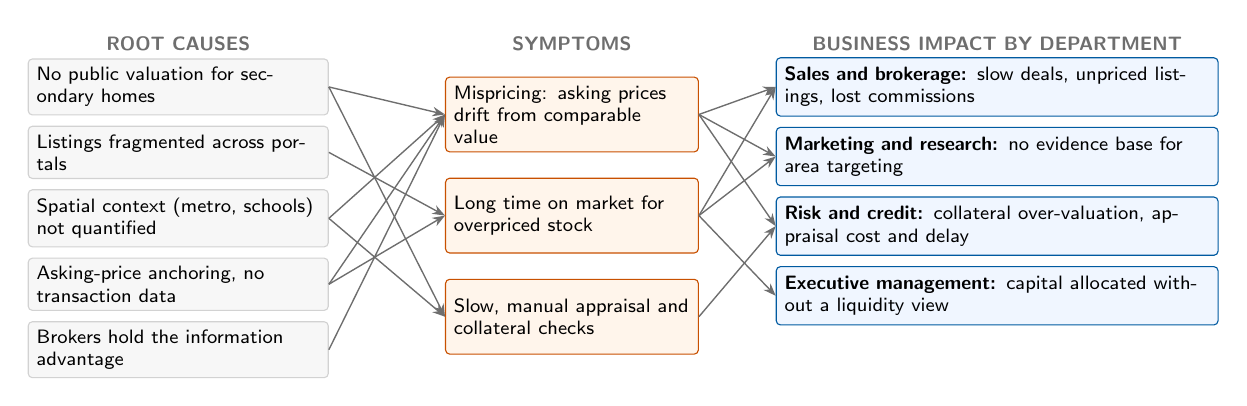
\begin{tikzpicture}[
  font=\sffamily\scriptsize,
  rc/.style={rounded corners=1.5pt, fill=lightgray, draw=rulecolor, text width=3.6cm, minimum height=0.62cm, align=left, inner sep=3pt},
  sy/.style={rounded corners=1.5pt, fill=orange!8!white, draw=accent, text width=3.0cm, minimum height=0.95cm, align=left, inner sep=3pt},
  im/.style={rounded corners=1.5pt, fill=metricbg, draw=brand, text width=5.4cm, minimum height=0.74cm, align=left, inner sep=3pt},
  hd/.style={font=\sffamily\bfseries\scriptsize, text=medgray},
  arr/.style={-{Stealth[length=1.6mm]}, color=medgray, line width=0.5pt}]
% root causes
\node[hd] at (0,0.55) {ROOT CAUSES};
\node[rc] (r1) at (0,0) {No public valuation for secondary homes};
\node[rc, below=0.13cm of r1] (r2) {Listings fragmented across portals};
\node[rc, below=0.13cm of r2] (r3) {Spatial context (metro, schools) not quantified};
\node[rc, below=0.13cm of r3] (r4) {Asking-price anchoring, no transaction data};
\node[rc, below=0.13cm of r4] (r5) {Brokers hold the information advantage};
% symptoms
\node[hd] at (5.0,0.55) {SYMPTOMS};
\node[sy] (s1) at (5.0,-0.35) {Mispricing: asking prices drift from comparable value};
\node[sy, below=0.32cm of s1] (s2) {Long time on market for overpriced stock};
\node[sy, below=0.32cm of s2] (s3) {Slow, manual appraisal and collateral checks};
% impact
\node[hd] at (10.4,0.55) {BUSINESS IMPACT BY DEPARTMENT};
\node[im] (i1) at (10.4,0) {\textbf{Sales and brokerage:} slow deals, unpriced listings, lost commissions};
\node[im, below=0.13cm of i1] (i2) {\textbf{Marketing and research:} no evidence base for area targeting};
\node[im, below=0.13cm of i2] (i3) {\textbf{Risk and credit:} collateral over-valuation, appraisal cost and delay};
\node[im, below=0.13cm of i3] (i4) {\textbf{Executive management:} capital allocated without a liquidity view};
\foreach \r in {r1,r4,r5} \draw[arr] (\r.east) -- (s1.west);
\foreach \r in {r2,r4} \draw[arr] (\r.east) -- (s2.west);
\foreach \r in {r1,r3} \draw[arr] (\r.east) -- (s3.west);
\draw[arr] (r3.east) -- (s1.west);
\draw[arr] (s1.east) -- (i1.west); \draw[arr] (s1.east) -- (i3.west);
\draw[arr] (s2.east) -- (i1.west); \draw[arr] (s2.east) -- (i4.west);
\draw[arr] (s3.east) -- (i3.west); \draw[arr] (s1.east) -- (i2.west); \draw[arr] (s2.east) -- (i2.west);
\end{tikzpicture} }
\end{column}
\end{columns}
\src{team analysis.}
\end{frame}

% 3 -------------------------------------------------------------- market
\begin{frame}{Existing tools cover project apartments or banks; the public, all-type quadrant is empty}
\begin{columns}[T]
\begin{column}{0.45\textwidth}
\resizebox{\textwidth}{!}{% ---- inlined from ../diagrams/positioning.tex ----
% Competitive positioning: x = property coverage, y = access (institutional -> public)
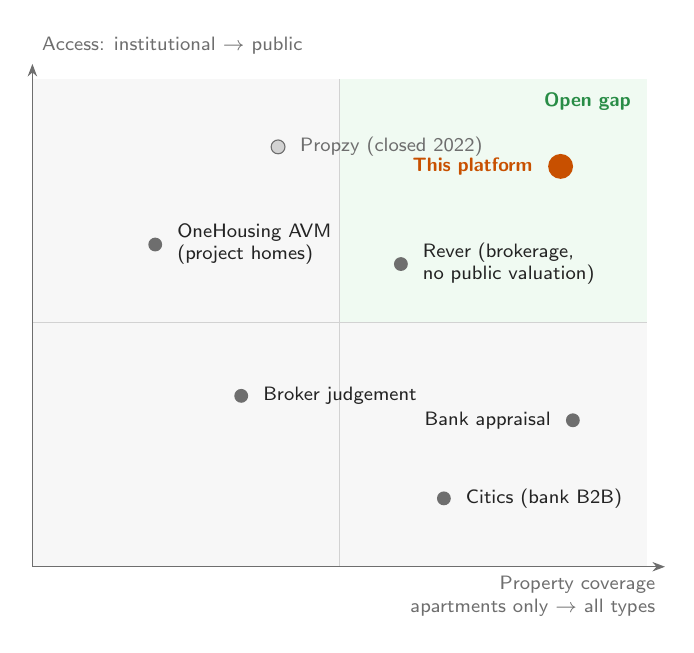
\begin{tikzpicture}[font=\sffamily\scriptsize, x=0.78cm, y=0.62cm,
  pl/.style={circle, inner sep=0pt, minimum size=5pt},
  lb/.style={font=\sffamily\scriptsize, text=darkgray, align=left}]
\fill[lightgray] (0,0) rectangle (10,10);
\fill[greenbg] (5,5) rectangle (10,10);
\draw[rulecolor] (5,0) -- (5,10); \draw[rulecolor] (0,5) -- (10,5);
\draw[-{Stealth[length=1.6mm]}, medgray] (0,0) -- (10.3,0) node[below left, text=medgray, align=right] {Property coverage\\apartments only $\rightarrow$ all types};
\draw[-{Stealth[length=1.6mm]}, medgray] (0,0) -- (0,10.3) node[above right, text=medgray] {Access: institutional $\rightarrow$ public};
\node[text=greenframe, font=\sffamily\bfseries\scriptsize, anchor=north east] at (9.9,9.9) {Open gap};
\node[pl, fill=medgray] at (2.0,6.6) {}; \node[lb, anchor=west] at (2.2,6.6) {OneHousing AVM\\(project homes)};
\node[pl, fill=medgray] at (6.7,1.4) {}; \node[lb, anchor=west] at (6.9,1.4) {Citics (bank B2B)};
\node[pl, fill=medgray] at (8.8,3.0) {}; \node[lb, anchor=east] at (8.6,3.0) {Bank appraisal};
\node[pl, fill=medgray] at (6.0,6.2) {}; \node[lb, anchor=west] at (6.2,6.2) {Rever (brokerage,\\no public valuation)};
\node[pl, fill=rulecolor, draw=medgray] at (4.0,8.6) {}; \node[lb, anchor=west, text=medgray] at (4.2,8.6) {Propzy (closed 2022)};
\node[pl, fill=medgray] at (3.4,3.5) {}; \node[lb, anchor=west] at (3.6,3.5) {Broker judgement};
\node[pl, fill=accent, minimum size=9pt] at (8.6,8.2) {}; \node[lb, anchor=east, font=\sffamily\bfseries\scriptsize, text=accent] at (8.3,8.2) {This platform};
\end{tikzpicture} }
\end{column}
\begin{column}{0.53\textwidth}
\small
\textbf{OneHousing:} 533,856 homes in 627 projects one month after its 2022 launch; company-reported error below 5\%; Techcombank partner.\\[4pt]
\textbf{Citics:} valuation used by more than 32 banks; USD 2.1 million raised in 2025; institutions only.\\[4pt]
\textbf{Rever:} brokerage, no public valuation. \textbf{Propzy:} closed in 2022.\\[6pt]
\colorbox{greenbg}{\parbox{0.95\textwidth}{\textbf{This platform:} all property types, published method, error stated by type, listings plus map data.}}
\end{column}
\end{columns}
\src{company pages and press reports (as reported, not independently verified); team positioning.}
\end{frame}

% 4 -------------------------------------------------------------- PDMT
\begin{frame}{One picture: problem, data, method and tool lead to three decisions}
\vspace{0.6cm}
\resizebox{\textwidth}{!}{% ---- inlined from ../diagrams/pdmt.tex ----
% PDMT map: Problem -> Data -> Method -> Tool -> Decision
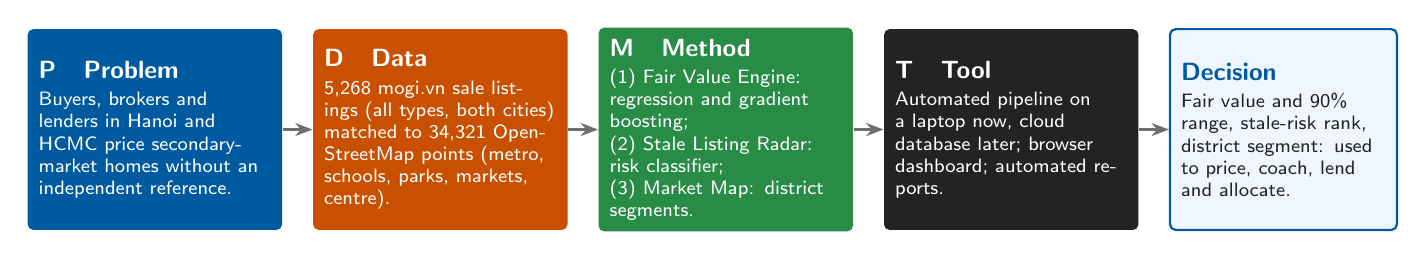
\begin{tikzpicture}[
  font=\sffamily\scriptsize,
  box/.style={draw=none, rounded corners=2pt, text width=2.95cm, minimum height=2.55cm, align=left, inner sep=4pt},
  head/.style={font=\sffamily\bfseries\small, text=white},
  arr/.style={-{Stealth[length=2.2mm]}, line width=1pt, color=medgray}]
\node[box, fill=brand] (P) {\textcolor{white}{\textbf{\small P\quad Problem}}\\[2pt]\textcolor{white}{Buyers, brokers and lenders in Hanoi and HCMC price secondary-market homes without an independent reference.}};
\node[box, fill=accent, right=0.38cm of P] (D) {\textcolor{white}{\textbf{\small D\quad Data}}\\[2pt]\textcolor{white}{\Nclean{} mogi.vn sale listings (all types, both cities) matched to \NpoiTotal{} OpenStreetMap points (metro, schools, parks, markets, centre).}};
\node[box, fill=greenframe, right=0.38cm of D] (M) {\textcolor{white}{\textbf{\small M\quad Method}}\\[2pt]\textcolor{white}{(1) Fair Value Engine: regression and gradient boosting;\\(2) Stale Listing Radar: risk classifier;\\(3) Market Map: district segments.}};
\node[box, fill=darkgray, right=0.38cm of M] (T) {\textcolor{white}{\textbf{\small T\quad Tool}}\\[2pt]\textcolor{white}{Automated pipeline on a laptop now, cloud database later; browser dashboard; automated reports.}};
\node[box, fill=metricbg, draw=brand, line width=0.8pt, right=0.38cm of T, text width=2.6cm] (B) {\textcolor{brand}{\textbf{\small Decision}}\\[2pt]\textcolor{darkgray}{Fair value and 90\% range, stale-risk rank, district segment: used to price, coach, lend and allocate.}};
\draw[arr] (P) -- (D); \draw[arr] (D) -- (M); \draw[arr] (M) -- (T); \draw[arr] (T) -- (B);
\end{tikzpicture} }
\src{team design; \srcmogi.}
\end{frame}

% 5 -------------------------------------------------------------- data
\begin{frame}{Two sources, one table: \Nclean{} listings matched to \NpoiTotal{} map points}
\centering\resizebox{0.86\textwidth}{!}{% ---- inlined from ../diagrams/architecture.tex ----
% Data architecture: sources -> raw store -> cleaning and location matching -> integrated table -> engines -> outputs
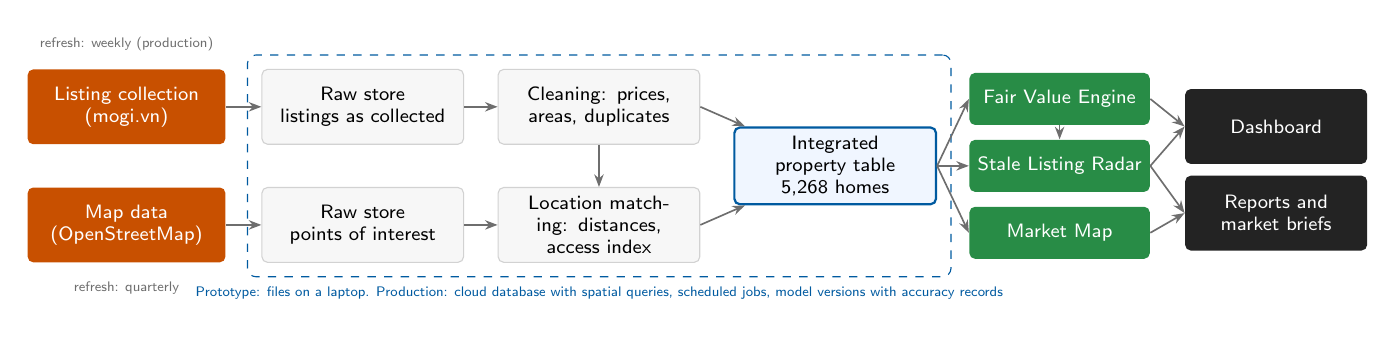
\begin{tikzpicture}[
  font=\sffamily\scriptsize,
  src/.style={rounded corners=2pt, fill=accent, text=white, text width=2.3cm, align=center, minimum height=0.95cm, inner sep=3pt},
  lay/.style={rounded corners=2pt, fill=lightgray, draw=rulecolor, text width=2.35cm, align=center, minimum height=0.95cm, inner sep=3pt},
  mod/.style={rounded corners=2pt, fill=greenframe, text=white, text width=2.15cm, align=center, minimum height=0.66cm, inner sep=2pt},
  outb/.style={rounded corners=2pt, fill=darkgray, text=white, text width=2.1cm, align=center, minimum height=0.95cm, inner sep=3pt},
  note/.style={font=\sffamily\tiny, text=medgray, align=center},
  arr/.style={-{Stealth[length=1.6mm]}, color=medgray, line width=0.6pt}]
\node[src] (m) at (0,0.75) {Listing collection\\(mogi.vn)};
\node[src] (o) at (0,-0.75) {Map data\\(OpenStreetMap)};
\node[lay] (raw) at (3.0,0.75) {Raw store\\listings as collected};
\node[lay] (cache) at (3.0,-0.75) {Raw store\\points of interest};
\node[lay] (cl) at (6.0,0.75) {Cleaning: prices, areas, duplicates};
\node[lay] (sj) at (6.0,-0.75) {Location matching: distances, access index};
\node[lay, fill=metricbg, draw=brand, line width=0.8pt] (tab) at (9.0,0) {Integrated property table\\ \Nclean{} homes};
\node[mod] (m1) at (11.85,0.85) {Fair Value Engine};
\node[mod] (m2) at (11.85,0) {Stale Listing Radar};
\node[mod] (m3) at (11.85,-0.85) {Market Map};
\node[outb] (dash) at (14.6,0.5) {Dashboard};
\node[outb] (rep) at (14.6,-0.6) {Reports and market briefs};
\draw[arr] (m) -- (raw); \draw[arr] (o) -- (cache); \draw[arr] (raw) -- (cl); \draw[arr] (cache) -- (sj);
\draw[arr] (cl) -- (sj); \draw[arr] (cl.east) -- (tab); \draw[arr] (sj.east) -- (tab);
\draw[arr] (tab.east) -- (m1.west); \draw[arr] (tab.east) -- (m2.west); \draw[arr] (tab.east) -- (m3.west);
\draw[arr] (m1) -- (m2);
\draw[arr] (m1.east) -- (dash.west); \draw[arr] (m2.east) -- (dash.west); \draw[arr] (m3.east) -- (rep.west); \draw[arr] (m2.east) -- (rep.west);
\node[note] at (0,1.55) {refresh: weekly (production)};
\node[note] at (0,-1.55) {refresh: quarterly};
\begin{scope}[on background layer]
\node[fit=(raw)(cache)(cl)(sj)(tab), draw=brand, dashed, rounded corners=3pt, inner sep=5pt] (prod) {};
\end{scope}
\node[note, text=brand, anchor=north] at (prod.south) {Prototype: files on a laptop. Production: cloud database with spatial queries, scheduled jobs, model versions with accuracy records};
\end{tikzpicture} }\\[0.15cm]
\raggedright\small
A prototype sample sized for a 1.5-hour collection window: \Nraw{} listings in \scrapeMinutes{} minutes (\throughput{} an hour, no blocks); \cleanShare{} survive cleaning. A scheduled run covers the full market (at least \supplyTotal{} listings) in about \fullRunHours{} hours.
\src{\srcmogi; \srcosm.}
\end{frame}

% 6 -------------------------------------------------------------- pipeline
\begin{frame}{Three linked engines turn one table into three decisions}
\vspace{0.3cm}
\centering\resizebox{0.86\textwidth}{!}{% ---- inlined from ../diagrams/pipeline.tex ----
% Analytical pipeline: how the three engines connect and which decision each feeds
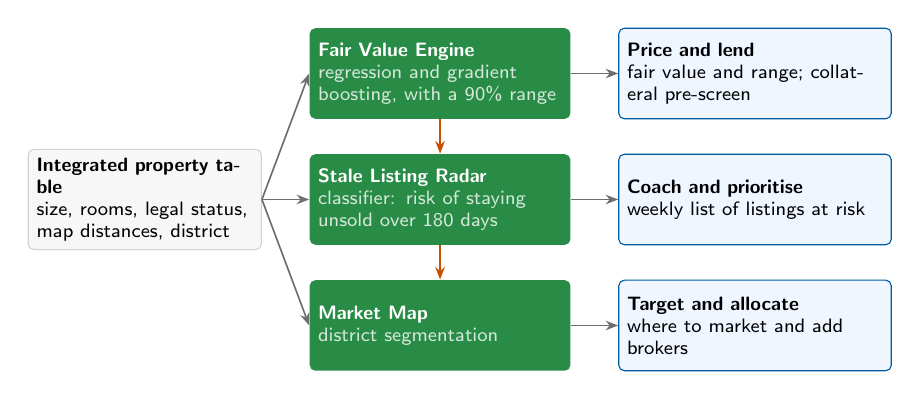
\begin{tikzpicture}[
  font=\sffamily\scriptsize,
  st/.style={rounded corners=2pt, fill=lightgray, draw=rulecolor, text width=2.75cm, align=left, minimum height=1.15cm, inner sep=3pt},
  md/.style={rounded corners=2pt, fill=greenframe, text=white, text width=3.1cm, align=left, minimum height=1.15cm, inner sep=3pt},
  dc/.style={rounded corners=2pt, fill=metricbg, draw=brand, text width=3.25cm, align=left, minimum height=1.15cm, inner sep=3pt},
  arr/.style={-{Stealth[length=1.6mm]}, color=medgray, line width=0.6pt}]
\node[st] (in) at (0,0) {\textbf{Integrated property table}\\size, rooms, legal status, map distances, district};
\node[md] (m1) at (3.75,1.6) {\textbf{Fair Value Engine}\\{\color{white!80!greenframe}regression and gradient boosting, with a 90\% range}};
\node[md] (m2) at (3.75,0) {\textbf{Stale Listing Radar}\\{\color{white!80!greenframe}classifier: risk of staying unsold over \staleDays{} days}};
\node[md] (m3) at (3.75,-1.6) {\textbf{Market Map}\\{\color{white!80!greenframe}district segmentation}};
\node[dc] (d1) at (7.75,1.6) {\textbf{Price and lend}\\fair value and range; collateral pre-screen};
\node[dc] (d2) at (7.75,0) {\textbf{Coach and prioritise}\\weekly list of listings at risk};
\node[dc] (d3) at (7.75,-1.6) {\textbf{Target and allocate}\\where to market and add brokers};
\draw[arr] (in.east) -- (m1.west); \draw[arr] (in.east) -- (m2.west); \draw[arr] (in.east) -- (m3.west);
\draw[arr, color=accent, line width=0.9pt] (m1.south) -- (m2.north);
\draw[arr, color=accent, line width=0.9pt] (m2.south) -- (m3.north);
\draw[arr] (m1) -- (d1); \draw[arr] (m2) -- (d2); \draw[arr] (m3) -- (d3);
\end{tikzpicture} }\\[0.3cm]
\raggedright\small Every accuracy figure comes from homes the engines had not seen. Listing age is measured from creation, because sellers refresh posted dates (\shareRefreshed{} re-posted after 30 days).
\src{team design.}
\end{frame}

% 7 -------------------------------------------------------------- Fair Value Engine
\begin{frame}{Fair Value Engine: \xgbPPEtwenty{} of unseen homes within ±20\%, better than regression on every measure}
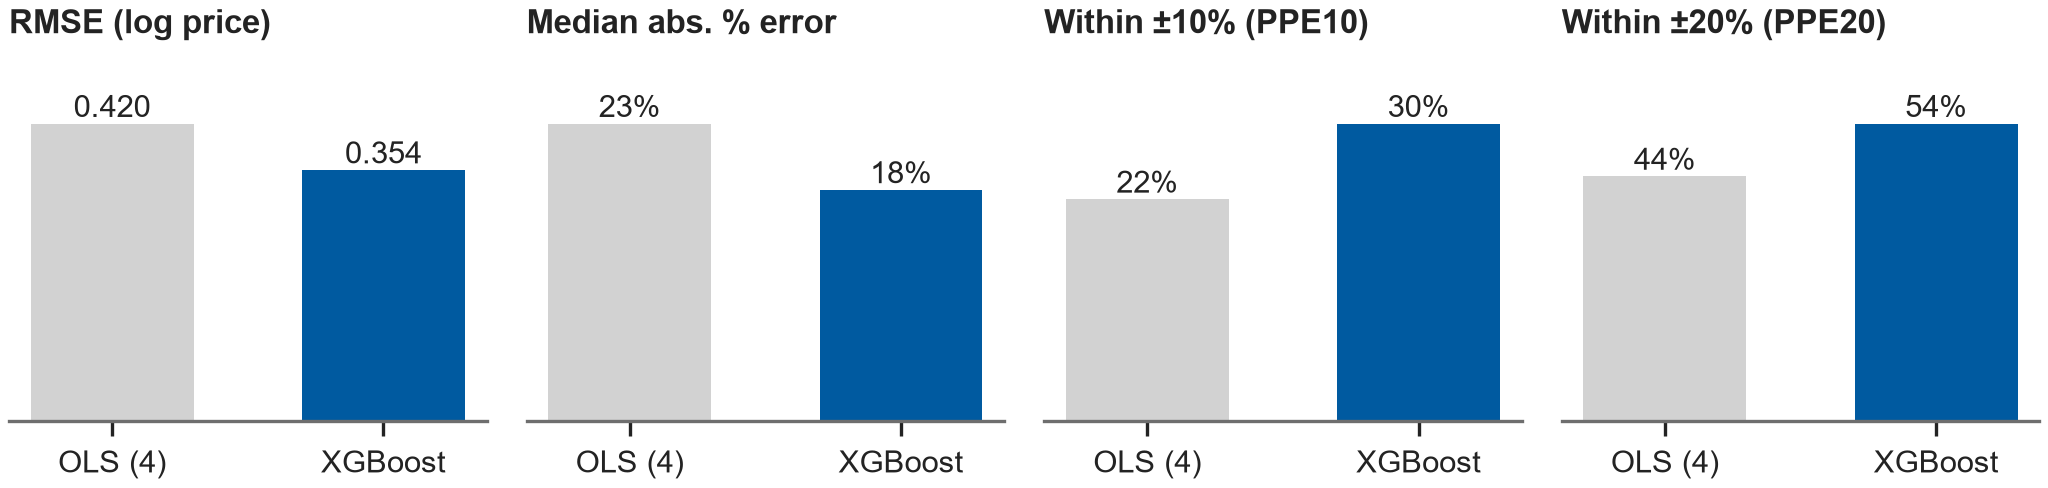
\includegraphics[width=\textwidth]{avm_performance.png}\\[0.2cm]
\small
\begin{columns}[T]
\begin{column}{0.5\textwidth}
\begin{itemize}
\item Ready for brokers: alley houses \ppeTwentyAlleyHouse, apartments \ppeTwentyApartment{} within ±20\%.
\item Not yet: street-front houses \ppeTwentyStreetFrontHouse, land \ppeTwentyLand.
\end{itemize}
\end{column}
\begin{column}{0.5\textwidth}
\begin{itemize}
\item Half of estimates miss by more than \xgbMdAPE: always show the 90\% range.
\item Typical error target of 0.20 (log scale) missed at \xgbRMSE.
\end{itemize}
\end{column}
\end{columns}
\src{\srcmogi; \Ntest{} test homes the models had not seen.}
\end{frame}

% 8 -------------------------------------------------------------- map data
\begin{frame}{Map data alone delivers \shareOSMofFE{} of the accuracy gain from knowing the district}
\begin{columns}[T]
\begin{column}{0.55\textwidth}
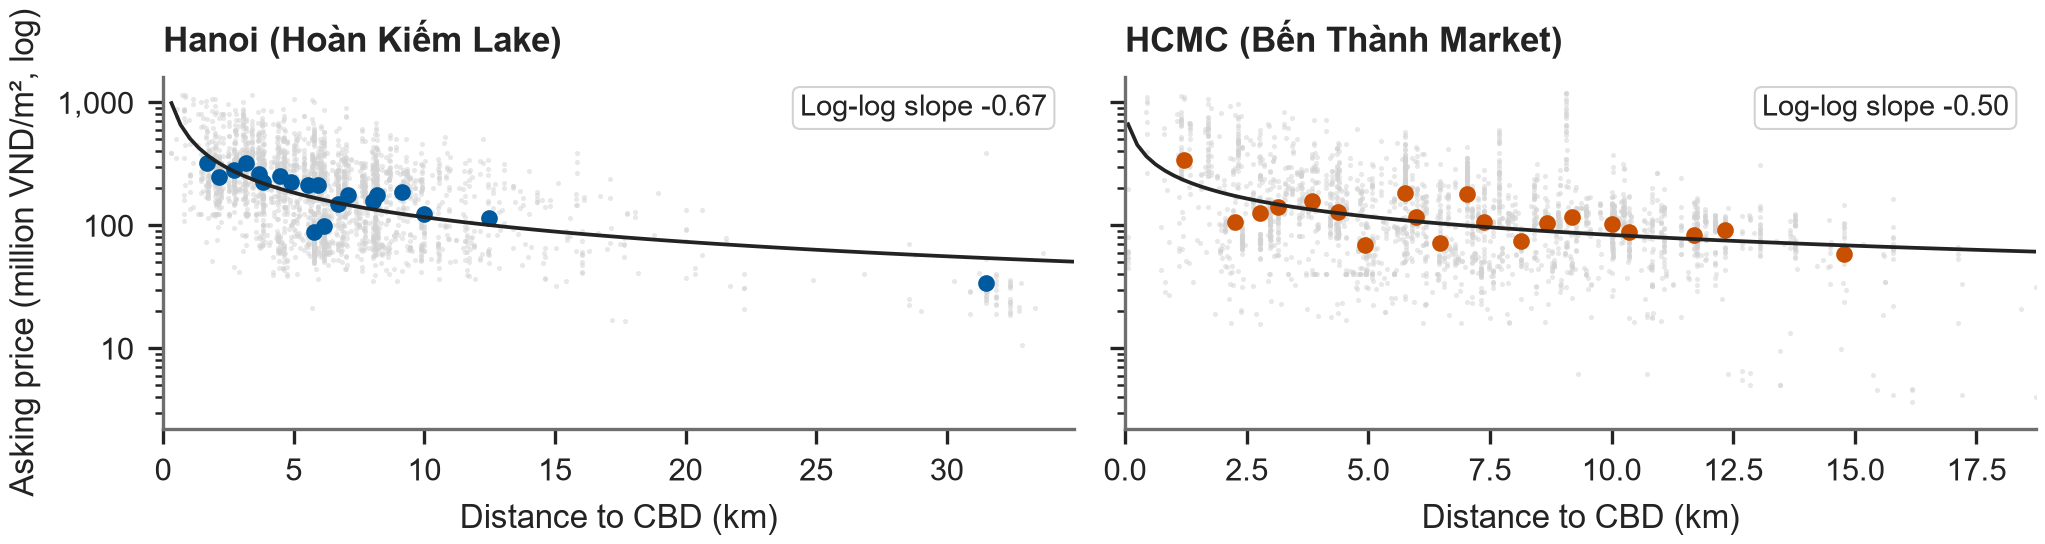
\includegraphics[width=\textwidth]{ppm2_vs_cbd.png}
\end{column}
\begin{column}{0.43\textwidth}
\small
\begin{itemize}
\item Size, rooms, legal status: R$^2$ \RtwoA.
\item Adding the district cuts the error by \cutDistrict.
\item Map distances without the district cut it by \cutOSMnoFE.
\item So the engine can value homes in districts with few listings.
\end{itemize}
\end{column}
\end{columns}
\src{\srcmogi; \srcosm; regression on log asking price, cross-validated error.}
\end{frame}

% 9 -------------------------------------------------------------- Stale Listing Radar
\begin{frame}{Stale Listing Radar: the top 10\% are stale \topDecileLift{} times as often as average, and price is not the driver}
\begin{columns}[T]
\begin{column}{0.62\textwidth}
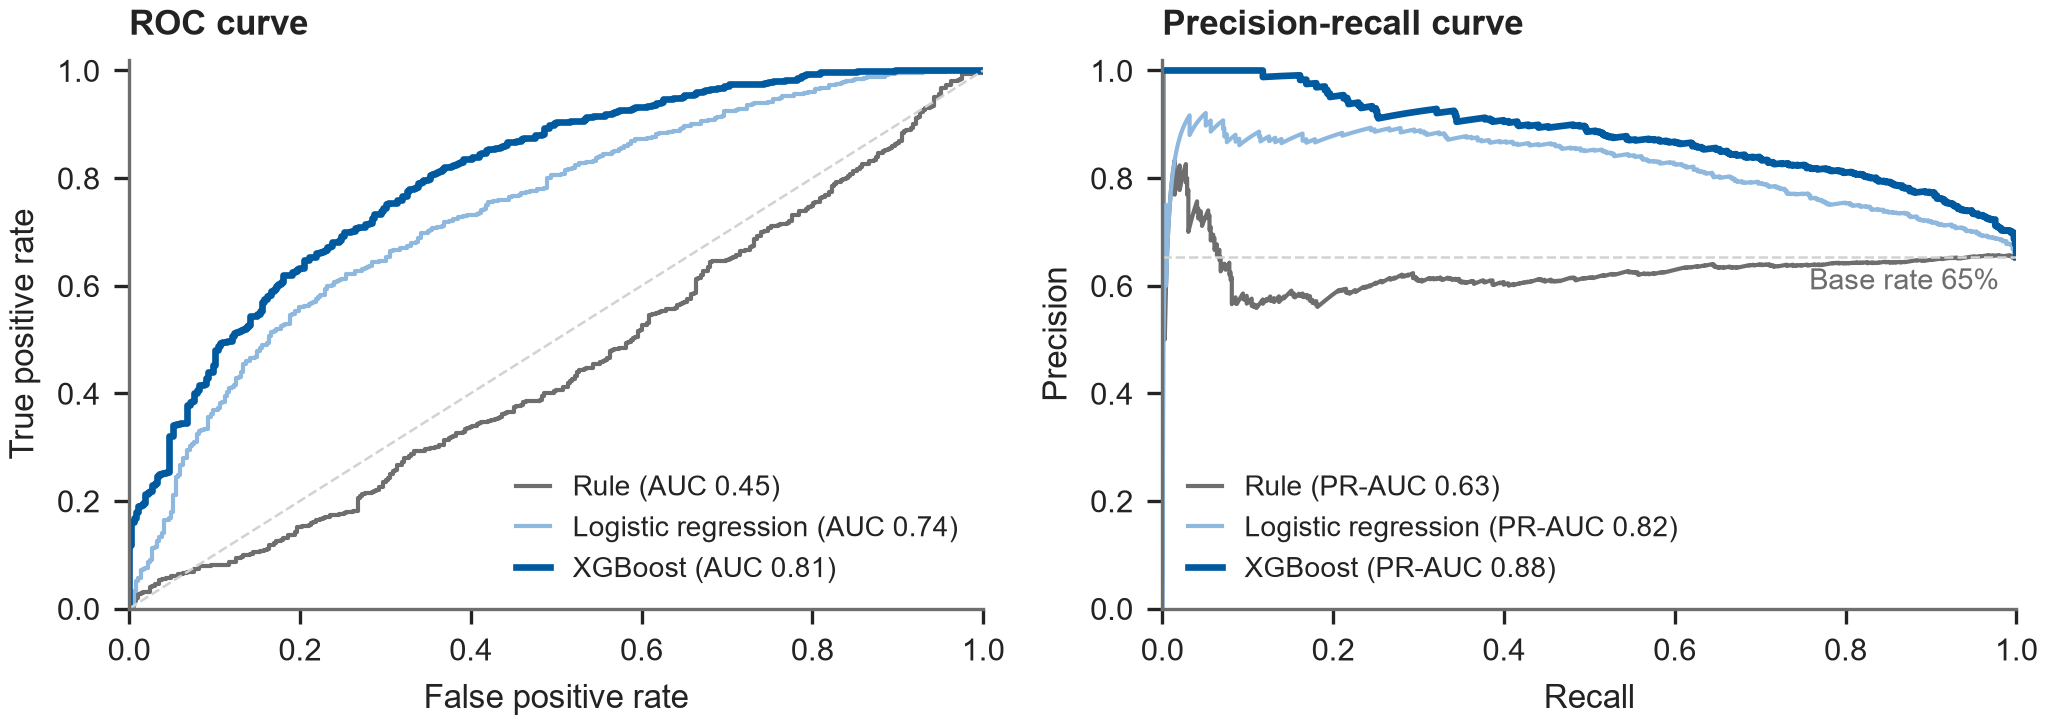
\includegraphics[width=\textwidth]{stale_roc_pr.png}
\end{column}
\begin{column}{0.36\textwidth}
\small
\begin{itemize}
\item AUC \xgbAUC{} (0.5 = coin flip); stale = unsold over \staleDays{} days.
\item Top 10\%: \topDecilePrecision{} stale against \baseRate{} on average.
\item A price-gap rule is no better than a coin flip; the gap ranks \residRank{} of \NstaleFeatures{} drivers.
\item Use the radar to target effort, the price gap to coach sellers.
\end{itemize}
\end{column}
\end{columns}
\src{\srcmogi; \NstaleTest{} test listings.}
\end{frame}

% 10 -------------------------------------------------------------- Market Map
\begin{frame}{Market Map: four district segments, four different messages}
\begin{columns}[T]
\begin{column}{0.64\textwidth}
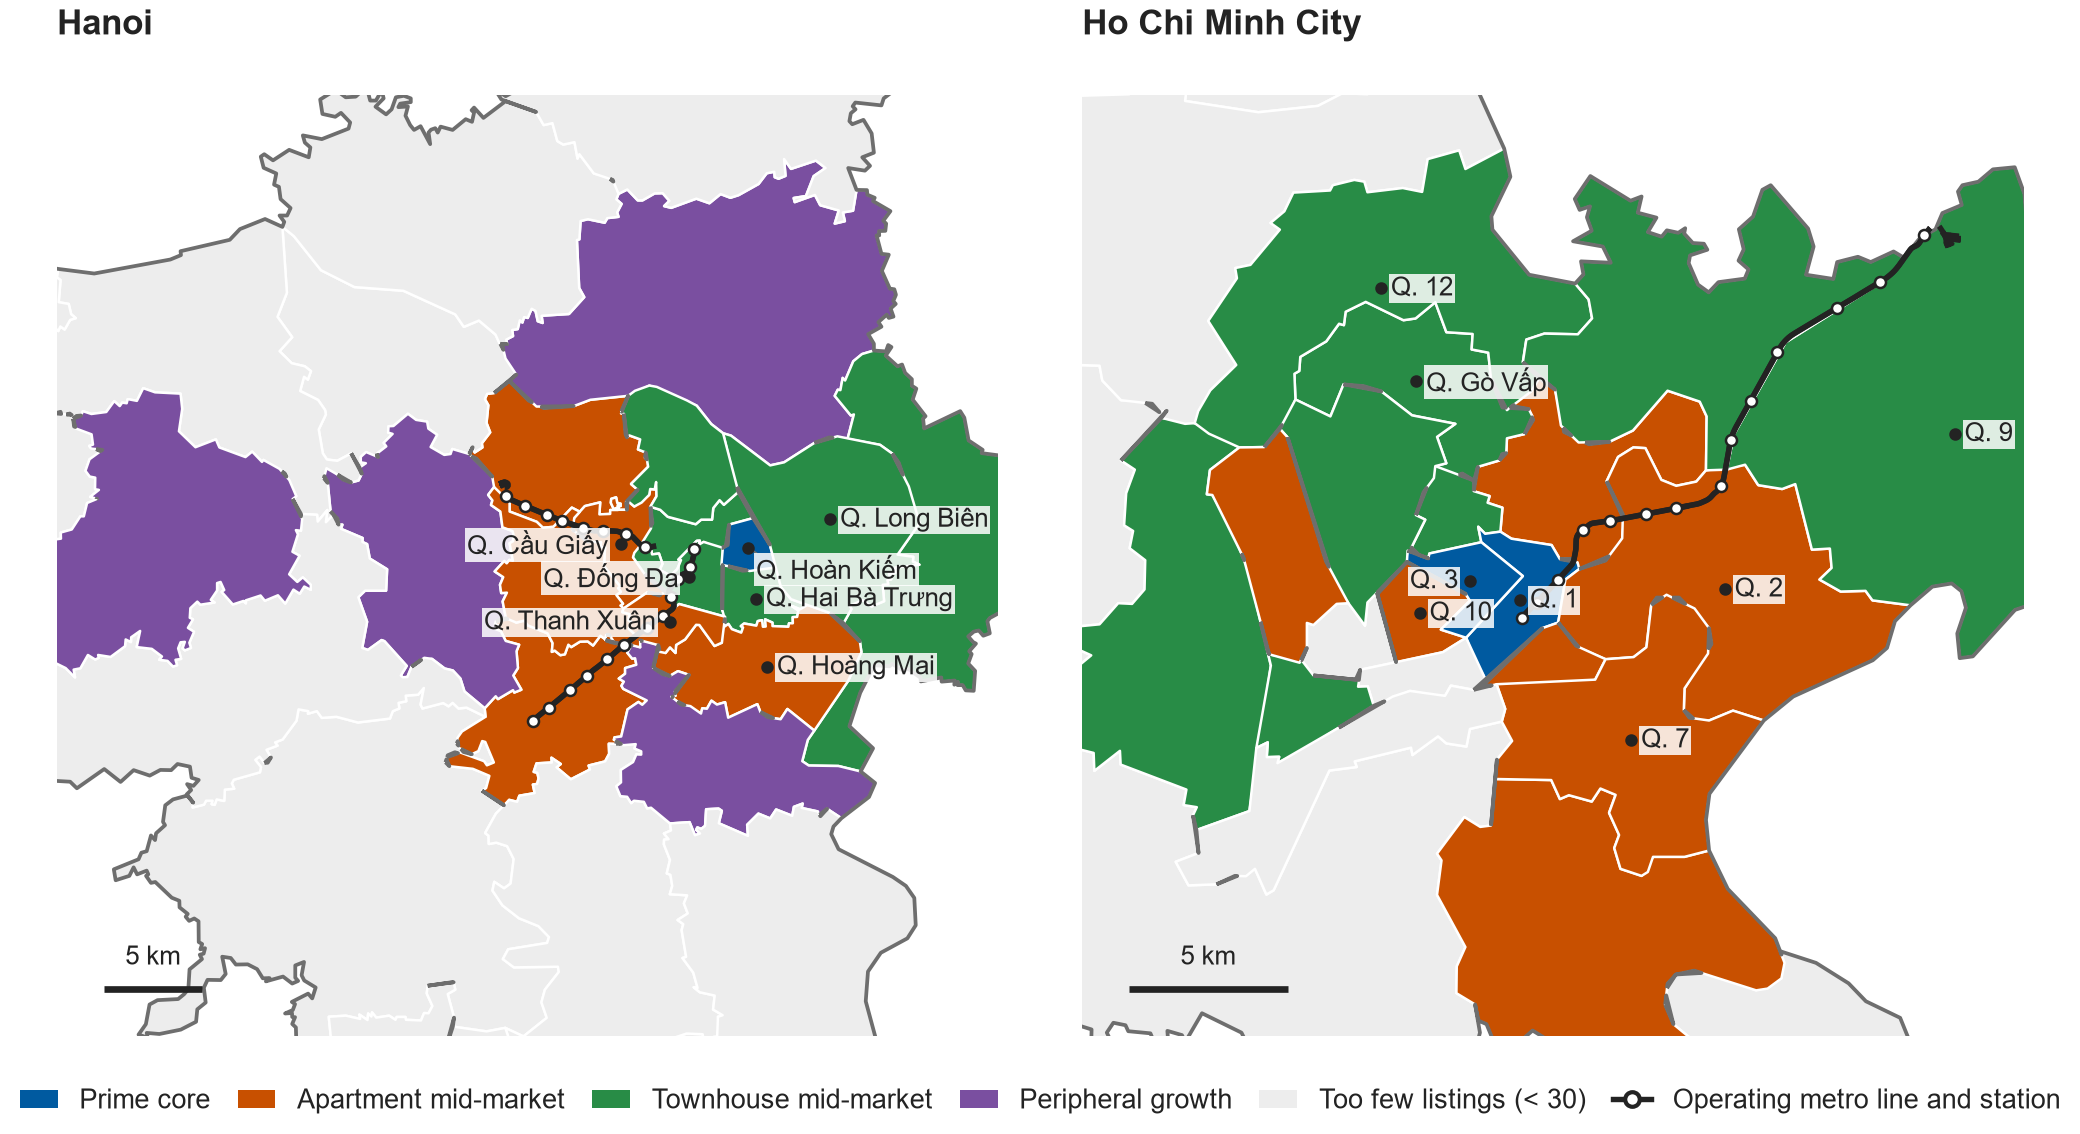
\includegraphics[width=\textwidth]{segments_maps.png}
\end{column}
\begin{column}{0.34\textwidth}
\small
\textbf{\segAname:} \segAppm{} m VND/m$^2$; defend price.\\[3pt]
\textbf{\segBname:} slowest (\segBage{} days); push harder.\\[3pt]
\textbf{\segCname:} fastest (\segCage{} days); volume.\\[3pt]
\textbf{\segDname:} land-led, highest stale risk (\segDrisk).\\[5pt]
{\color{medgray}Segments overlap: use them as targeting groups, not hard borders.}
\end{column}
\end{columns}
\src{\srcmogi; \srcosm; district boundaries GADM 4.1.}
\end{frame}

% 11 -------------------------------------------------------------- departments
\begin{frame}{Every department gets a decision tool and a KPI}
\small
\begin{tabularx}{\textwidth}{@{}>{\bfseries}p{2.6cm}XXp{3.6cm}@{}}
\toprule
Department & Decision & Evidence & KPI \\
\midrule
Sales and brokerage & Which listings to prioritise, which sellers to coach & Top-quarter risk share: \topRiskShare{} in \topRiskDistrict; \overFifteenStreetFrontHouse{} of street-front houses ask $>$15\% above fair value & Days to sale, coached vs not \\
Marketing and research & Which areas, which message & Four segments differ in price, speed and mix & Leads per listing by segment \\
Risk and credit & When a fair value can pre-screen collateral & Fair value exceeds the asking price by $>$20\% for \overAll{} of homes; desk review needed & Pre-screens confirmed within ±10\% \\
Executive management & Where to add brokers and offices & Speed vs price matrix by district & Median listing age by segment \\
\bottomrule
\end{tabularx}
\src{team analysis.}
\end{frame}

% 12 -------------------------------------------------------------- value
\begin{frame}{Base case: VND \netPartnerBase{} bn net partner value a year, \roiBase{} times the run cost; adoption decides}
\begin{columns}[T]
\begin{column}{0.62\textwidth}
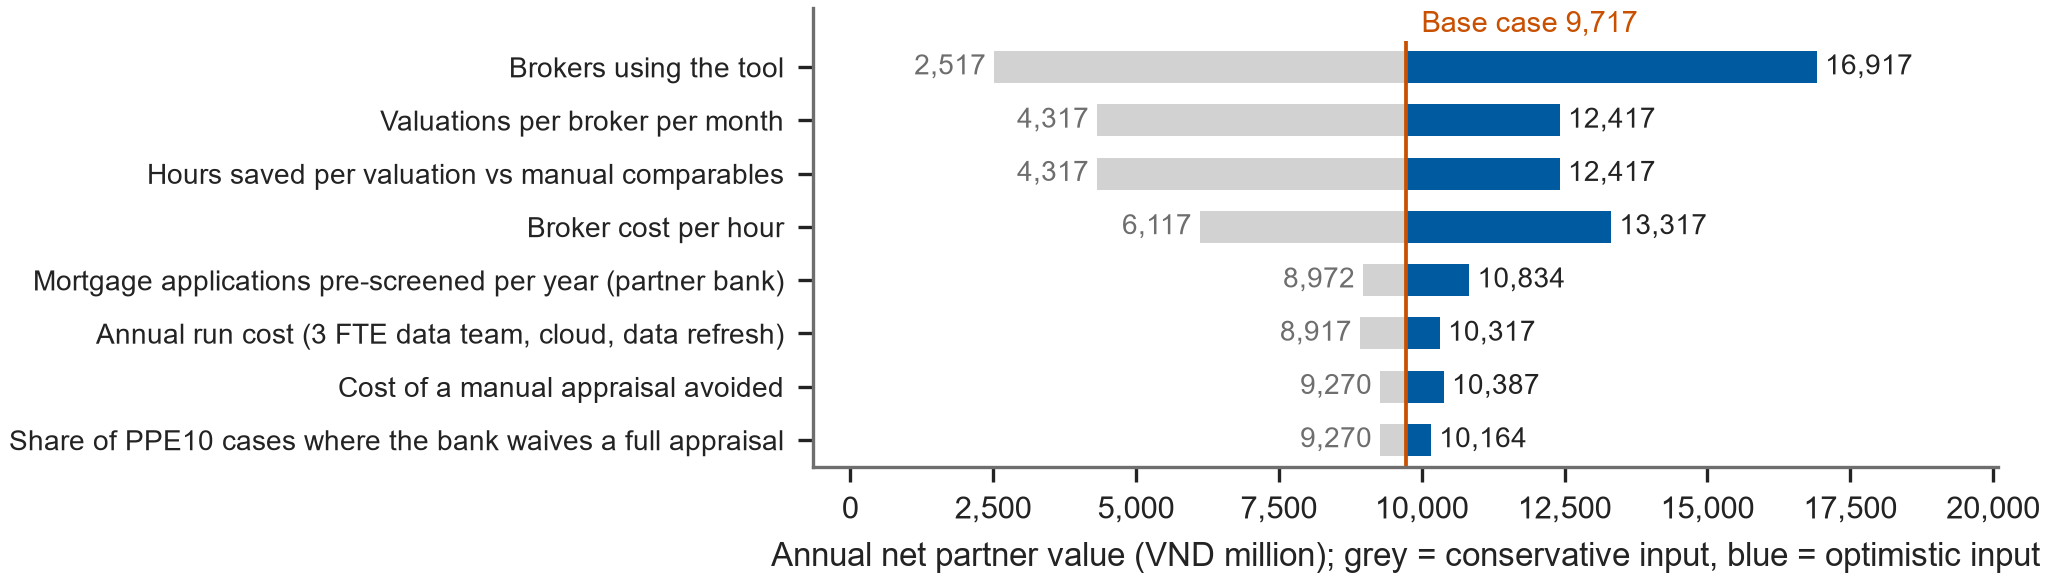
\includegraphics[width=\textwidth]{value_tornado.png}
\end{column}
\begin{column}{0.36\textwidth}
\small
\begin{itemize}
\item Partner value VND \partnerBase{} bn against a run cost of \runCostBase{} bn.
\item Range: VND \netPartnerCons{} to \netPartnerOpt{} bn a year.
\item Buyers save VND \buyerBase{} bn (outside the ROI).
\item Scenario estimates on labelled assumptions, not measured outcomes.
\end{itemize}
\end{column}
\end{columns}
\src{team assumptions; partner value = broker time saved + bank appraisals avoided.}
\end{frame}

% 13 -------------------------------------------------------------- roadmap
\begin{frame}[fragile]{Twelve months, three phases, a go or no-go gate at each step}
\centering\resizebox{0.9\textwidth}{!}{% ---- inlined from ../diagrams/roadmap.tex ----
% Implementation roadmap (Gantt style), months 1 to 12.
% Task names sit in a left column outside the timeline; bars start on the month grid; owners sit right of each bar;
% milestones sit on their own row below each phase.
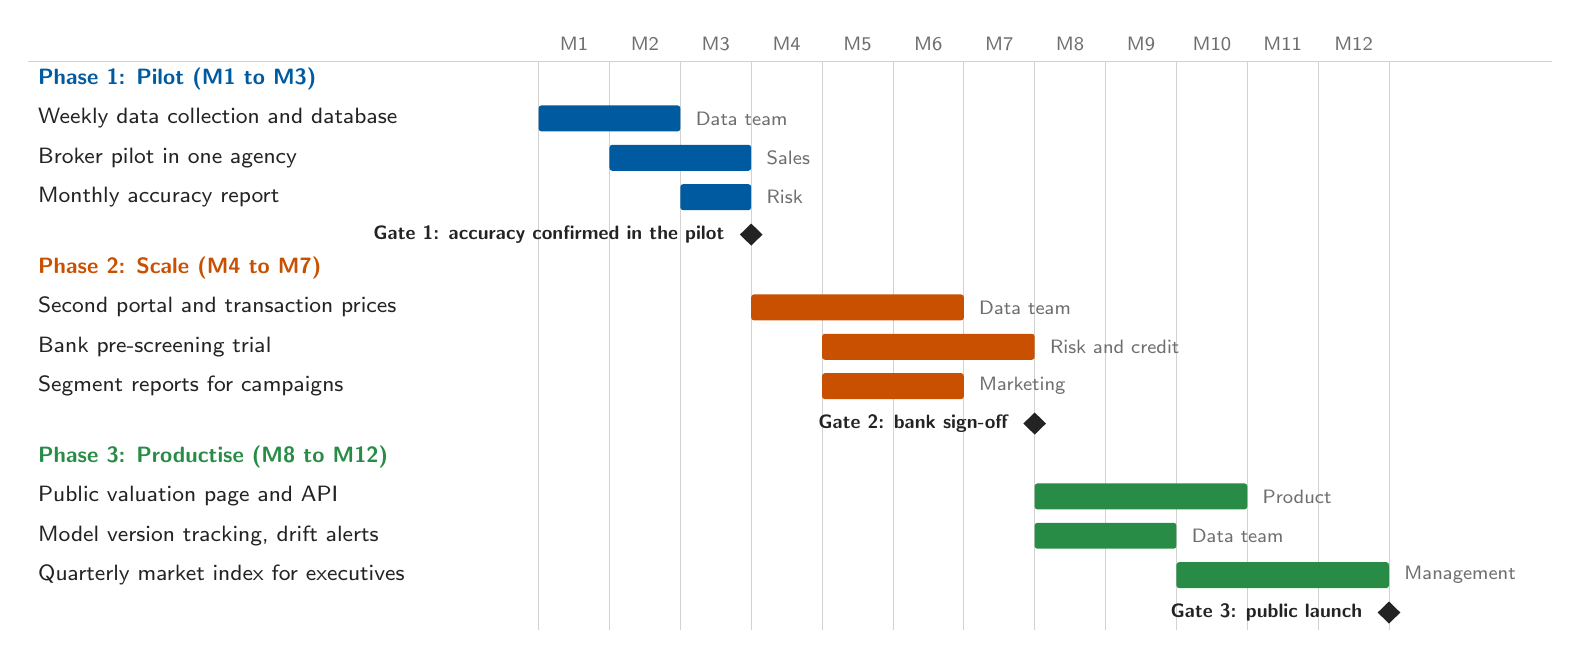
\begin{tikzpicture}[font=\sffamily\footnotesize, x=0.9cm, y=0.5cm]
\def\T{7.2}% x where month 1 starts
% month header and grid
\foreach \m in {1,...,12} { \node[text=medgray, font=\sffamily\scriptsize] at (\T+\m-0.5,0.9) {M\m}; }
\foreach \m in {0,...,12} { \draw[rulecolor, line width=0.3pt] (\T+\m,0.45) -- (\T+\m,-14.0); }
\draw[rulecolor, line width=0.5pt] (0,0.45) -- (\T+14.3,0.45);
% phase titles
\newcommand{\phase}[3]{\node[anchor=west, font=\sffamily\bfseries\footnotesize, text=#3] at (0,#1) {#2};}
\phase{0}{Phase 1: Pilot (M1 to M3)}{brand}
\phase{-4.8}{Phase 2: Scale (M4 to M7)}{accent}
\phase{-9.6}{Phase 3: Productise (M8 to M12)}{greenframe}
% task: y, name, start month (0-based), end month, colour, owner
\newcommand{\task}[6]{%
  \node[anchor=west, text=darkgray] at (0,#1) {#2};
  \fill[#5, rounded corners=1pt] (\T+#3,#1-0.33) rectangle (\T+#4,#1+0.33);
  \node[anchor=west, text=medgray, font=\sffamily\scriptsize] at (\T+#4+0.08,#1) {#6};}
\task{-1}{Weekly data collection and database}{0}{2}{brand}{Data team}
\task{-2}{Broker pilot in one agency}{1}{3}{brand}{Sales}
\task{-3}{Monthly accuracy report}{2}{3}{brand}{Risk}
\task{-5.8}{Second portal and transaction prices}{3}{6}{accent}{Data team}
\task{-6.8}{Bank pre-screening trial}{4}{7}{accent}{Risk and credit}
\task{-7.8}{Segment reports for campaigns}{4}{6}{accent}{Marketing}
\task{-10.6}{Public valuation page and API}{7}{10}{greenframe}{Product}
\task{-11.6}{Model version tracking, drift alerts}{7}{9}{greenframe}{Data team}
\task{-12.6}{Quarterly market index for executives}{9}{12}{greenframe}{Management}
% milestones: diamond on the month boundary, label to its left on a free row
\newcommand{\milestone}[3]{%
  \fill[darkgray] (\T+#1,#2+0.28) -- (\T+#1+0.16,#2) -- (\T+#1,#2-0.28) -- (\T+#1-0.16,#2) -- cycle;
  \node[anchor=east, text=darkgray, font=\sffamily\scriptsize\bfseries] at (\T+#1-0.24,#2) {#3};}
\milestone{3}{-3.95}{Gate 1: accuracy confirmed in the pilot}
\milestone{7}{-8.75}{Gate 2: bank sign-off}
\milestone{12}{-13.55}{Gate 3: public launch}
\end{tikzpicture} }
\src{team plan.}
\end{frame}

% 14 -------------------------------------------------------------- risks and asks
\begin{frame}{Risks are known and owned; three asks to start the pilot}
\begin{columns}[T]
\begin{column}{0.5\textwidth}
\small\textbf{Top risks and mitigations}
\begin{itemize}
\item Asking vs transaction price: calibrate on bank appraisals in Phase 2.
\item Noisy stale label: weekly data collection gives true time to sale.
\item Site changes: tested page readers, a second portal.
\item Publishing valuations: ranges, disclaimers, published method.
\end{itemize}
\end{column}
\begin{column}{0.48\textwidth}
\small\textbf{Asks}
\begin{enumerate}
\item One brokerage partner for a 3-month pilot (apartments, alley houses).
\item Appraisal or notarised prices from a partner bank.
\item Budget for a 3-person data team (VND \runCostBase{} bn a year, base case).
\end{enumerate}
\end{column}
\end{columns}
\src{team analysis.}
\end{frame}

% 15 -------------------------------------------------------------- appendix
\begin{frame}{Appendix: a pricing reference for brokers today, not yet a lending tool}
\begin{columns}[T]
\begin{column}{0.5\textwidth}
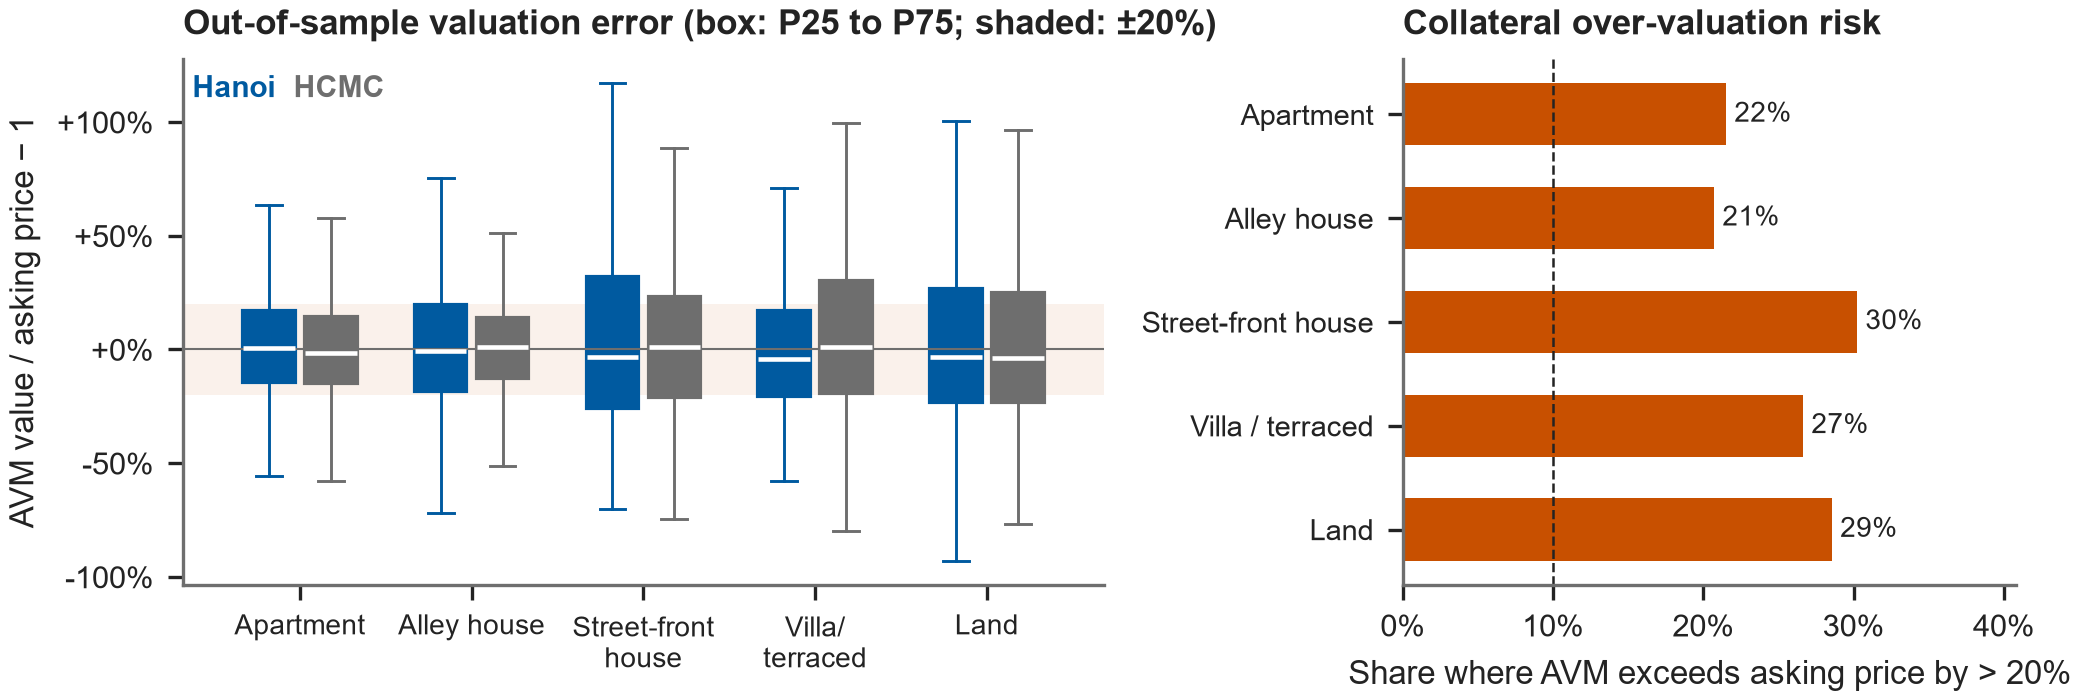
\includegraphics[width=\textwidth]{xf_risk.png}
\end{column}
\begin{column}{0.48\textwidth}
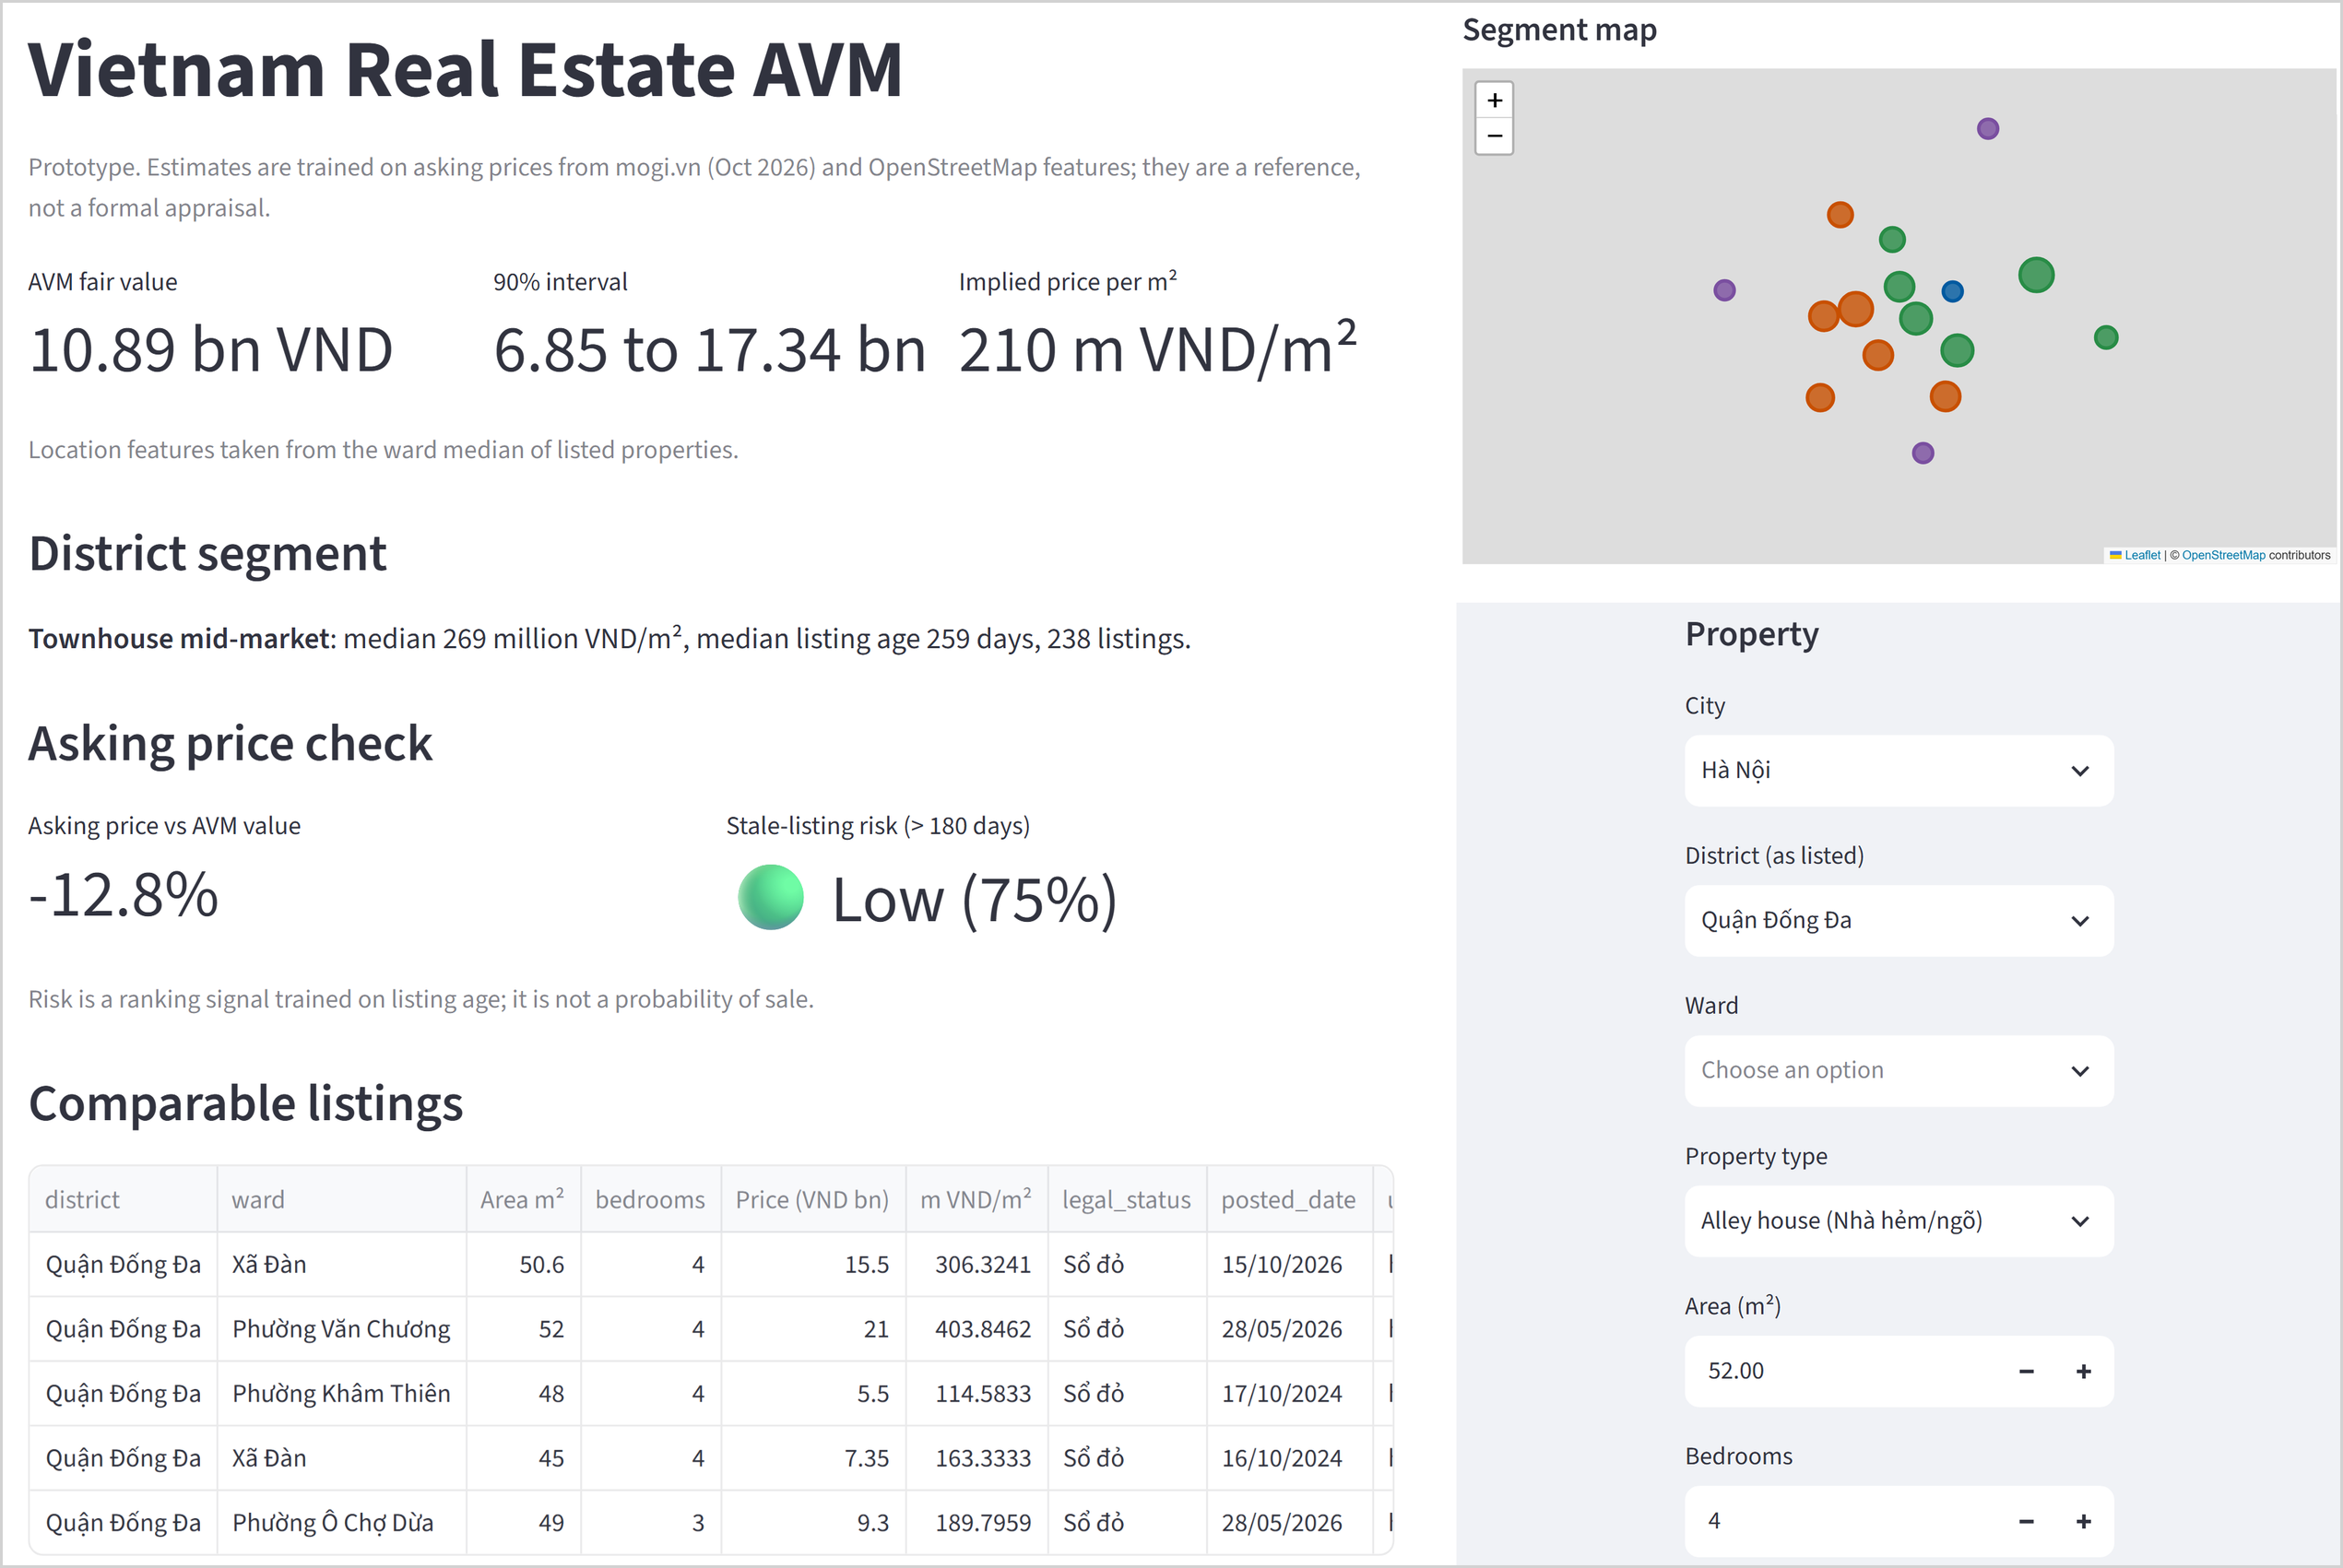
\includegraphics[width=\textwidth]{dashboard_screenshot.png}
\end{column}
\end{columns}
\small Expensive homes tend to be under-valued; monitor before any lending use. The dashboard shows fair value, range, price gap, stale-risk light and comparables.
\src{\srcmogi; dashboard prototype.}
\end{frame}

\end{document}
